\section{Вычисления}
\subsection{Пример вычисления}
Для \(N = 20\) рассматривается выборка точек с ее содержимым:

\begin{align*}
	\begin{array}{ll}
		(0.56763554 0.0789485) \to 457.23883   & (0.74630606 0.6721467) \to 788.1961   \\
		(0.43813038 0.57967687) \not\in D      & (0.34509814 0.5507567) \not\in D      \\
		(0.14233947 0.4783113) \not\in D       & (0.032078028 0.31770563) \not\in D    \\
		(0.8451768 0.15828753) \to 588.081     & (0.37217999 0.48739147) \to 576.4103  \\
		(0.48926282 0.085366964) \to 433.40872 & (0.2324897 0.54943454) \not\in D      \\
		(0.8560116 0.7436471) \to 858.1829     & (0.4741887 0.977206) \not\in D        \\
		(0.6843517 0.65986276) \to 761.45844   & (0.79020524 0.92588997) \not\in D     \\
		(0.17501795 0.9010966) \not\in D       & (0.59115267 0.17000258) \to 506.70572 \\
		(0.51510084 0.84061956) \not\in D      & (0.8522557 0.82952595) \to 895.9853   \\
		(0.8507035 0.46353948) \to 728.8909    & (0.56606627 0.77454865) \not\in D     \\
	\end{array}
\end{align*}
\begin{align*}
	I = \frac{1}{20}\sum_{k=0}^{10}=\frac{1}{20}( & 457.23883+588.081+433.40872+                     \\
	+                                             & 858.1829+761.45844+728.8909+                     \\
	+                                             & 788.1961+576.4103+506.70572+895.9853) = 329.7279
\end{align*}

\subsection{Отклонения}
Взяв для каждой конфигурации, для каждого \(N\), выборки в количестве \(K\) с размером каждой выборки \(K_i = K_0\) производятся вычисления:
\begin{enumerate}
	\item Вычисляется нормальное отклонение для каждой выборки
	      \begin{align}
		      \sigma_i = \sqrt{\frac{1}{K_i}\sum_{j=0}^{K_i} (x_k - \overline{x})^2}, i=\overline{0,K}
	      \end{align}
	\item Находится среднее значение среди полученных нормальных отклонений:
	      \begin{align}
		      m_\sigma = \frac{1}{K}\sum_{i=0}^K \sigma_i
	      \end{align}
	\item А так же нормальное отклонение среди полученных:
	      \begin{align}
		      \sigma_\sigma = \sqrt{\frac{1}{K}\sum_{i=0}^K(\sigma - \sigma_i)^2}
	      \end{align}
\end{enumerate}
Для вычислений взяты значения \(K=30\), \(K_0=100\).
\begin{table}[h!]
	\centering
	\begin{tabular}{|l|c|c|c|c|c|}
		\hline
		$N$     & $m_{\sigma1}$ & $\sigma_{\sigma1}$ & $m_{\sigma2}$  & $\sigma_{\sigma2}$ \\
		\hline
		$  20 $ & $  74.08163 $ & $ 4.6014333 $      & $ 109.821976 $ & $  7.773065 $      \\
		$  50 $ & $  46.76052 $ & $ 3.2611177 $      & $    68.9947 $ & $ 4.8407636 $      \\
		$ 100 $ & $ 32.825172 $ & $   2.68074 $      & $  47.794693 $ & $ 3.8238974 $      \\
		$ 200 $ & $ 22.975714 $ & $  1.596667 $      & $  34.144722 $ & $ 3.1301556 $      \\
		$ 300 $ & $ 19.188334 $ & $ 1.2513237 $      & $  27.316946 $ & $ 2.0922694 $      \\
		$ 400 $ & $ 17.110592 $ & $ 1.4182564 $      & $  24.498312 $ & $ 1.6277343 $      \\
		$ 500 $ & $ 14.788441 $ & $ 0.9899412 $      & $  21.324444 $ & $ 1.7795098 $      \\
		\hline
	\end{tabular}
\end{table}
\begin{figure}[h!]
	\hspace{-2em}
	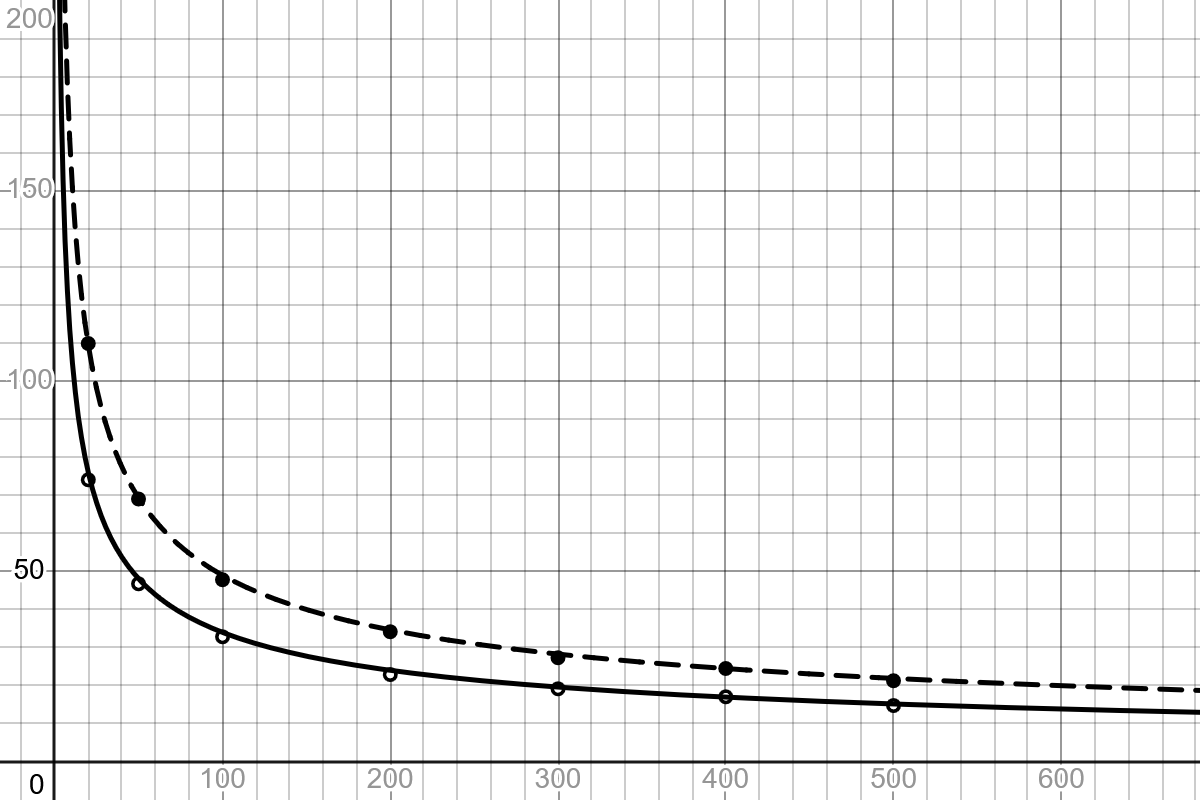
\includegraphics[width=\linewidth]{graphics/desmos-graph.png}
\end{figure}

% +-----+-----------+-----------+
% | N   | mₓ        | dₓ        |
% +-----+-----------+-----------+
% |  20 |  74.08163 | 4.6014333 |
% |  50 |  46.76052 | 3.2611177 |
% | 100 | 32.825172 |   2.68074 |
% | 200 | 22.975714 |  1.596667 |
% | 300 | 19.188334 | 1.2513237 |
% | 400 | 17.110592 | 1.4182564 |
% | 500 | 14.788441 | 0.9899412 |
% +-----+-----------+-----------+
% +-----+------------+-----------+
% | N   | mₓ         | dₓ        |
% +-----+------------+-----------+
% |  20 | 109.821976 |  7.773065 |
% |  50 |    68.9947 | 4.8407636 |
% | 100 |  47.794693 | 3.8238974 |
% | 200 |  34.144722 | 3.1301556 |
% | 300 |  27.316946 | 2.0922694 |
% | 400 |  24.498312 | 1.6277343 |
% | 500 |  21.324444 | 1.7795098 |
% +-----+------------+-----------+
